\title{Study Guide for Midterm 1}
\author{Dr. Jordan Hanson - Whittier College Dept. of Physics and Astronomy}
\date{\today}
\documentclass[10pt]{article}
\usepackage[a4paper, total={18cm, 27cm}]{geometry}
\usepackage{outlines}
\usepackage{graphicx}
\begin{document}
\maketitle

\section{Chapter 1 - Introductory Concepts}
\begin{figure}[ht]
\centering
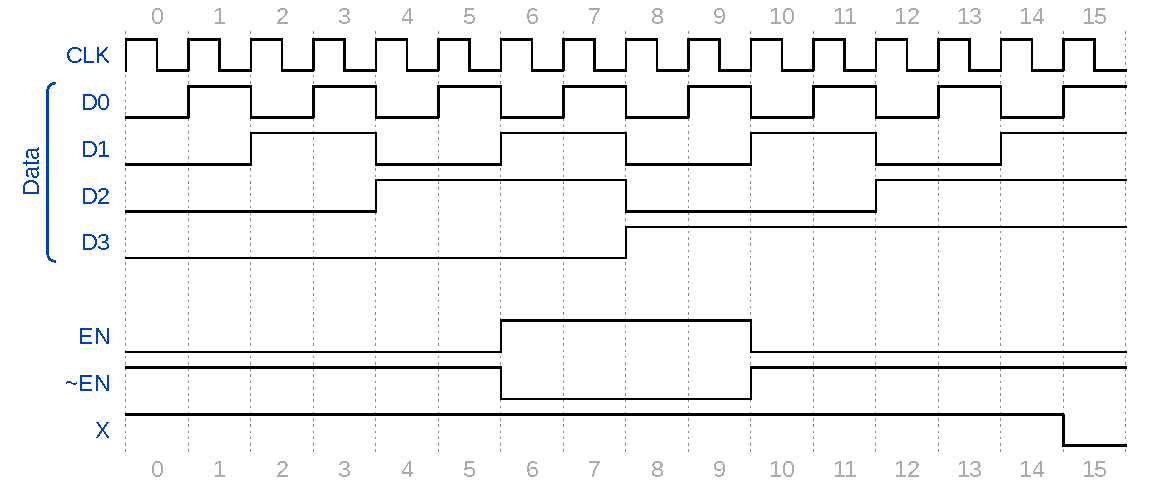
\includegraphics[width=0.6\textwidth]{timingExample7a.pdf}
\caption{\label{fig:timing7} A timing diagram including a clock signal (CLK), a 4-bit parallel data stream (D0-D3), and enable/disable signals (EN/$\sim$EN).}
\end{figure}
\begin{enumerate}
\item Consider Fig. \ref{fig:timing1}. (a) What is the duty cycle of each $D_{\rm i}$ signal? (b) Consider the bitstreams of $D_{\rm i}$.  What does the sequence of numbers represent?
\begin{itemize}
\item All duty cycles are 50\%
\item This is a 4-bit counter
\end{itemize}
\item (a) Imagine that $D_i$ signals enter a NAND gate, along with the $\sim$EN signal.  Draw the resulting timing diagram. \\ \\
\textit{See Fig. \ref{fig:timing7}, with the output X}.
\item Suppose $D_i$ represents parallel data with a clock frequency of 4 MHz.  (a) What is the total bitrate (bits per second)?  (b) What would be the bit rate if the system was serial instead of parallel?
\begin{itemize}
\item 16 Mbps (16 MHz)
\item 4 Mbps (4 MHz)
\end{itemize}
\end{enumerate}

\section{Chapter 2 - Number Systems, Operations, and Codes}

\begin{enumerate}
\item Convert to binary: (a) 1024 (decimal) (b) 0xBBBB (hex) (c) -2048 (decimal)
\begin{itemize}
\item 0100 0000 0000
\item 1011 1011 1011 1011
\item \textit{2's complement:} 1000 0000 0000 ... ends up the same representation unless you add leading 0's
\end{itemize}
\item Convert to hex: (a) 65535 (decimal) (b) 1000100010001000 (binary)
\begin{itemize}
\item 0xFFFF
\item 0x8888
\end{itemize}
\item Convert to \textit{octal}, in which \textbf{the base is 8}: 1024 (decimal)
\begin{itemize}
\item 0o2000
\end{itemize}
\item Consider the gray code angular encoder in Fig. \ref{fig:grayCode}.  (a) If the shaft rotates 180 degrees, how many bit changes occur?  (b) If it rotates 180 degrees, and the initial gray code is 0000, what is the final gray code?  (c) With 4-bit gray code, how many distinct angles can the shaft encode?  What is 360 degrees divided by this number (i.e. the angular precision)? (d) What would be the angular precision of an 8 bit encoder?
\begin{itemize}
\item 7 bit changes
\item 1000 (7 in gray code)
\item 16, 22.5 degrees
\item 1.4 degrees
\end{itemize}
\end{enumerate}
\begin{figure}[hb]
\centering
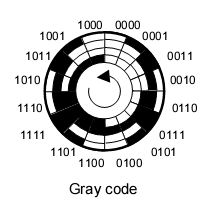
\includegraphics[width=0.15\textwidth]{grayCode1.png}
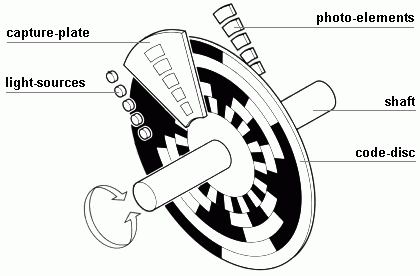
\includegraphics[width=0.25\textwidth]{grayCode2.png}
\caption{\label{fig:grayCode} A gray code shaft encoder, or angular encoder, reports the angular position of an object digitally, using the gray code.}
\end{figure}

\section{Chapter 3 - Logic Gates}
\begin{figure}[ht]
\centering
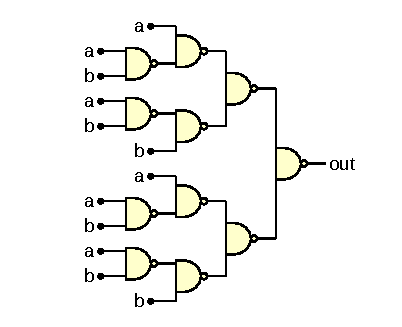
\includegraphics[width=0.25\textwidth]{gateExample5.pdf}
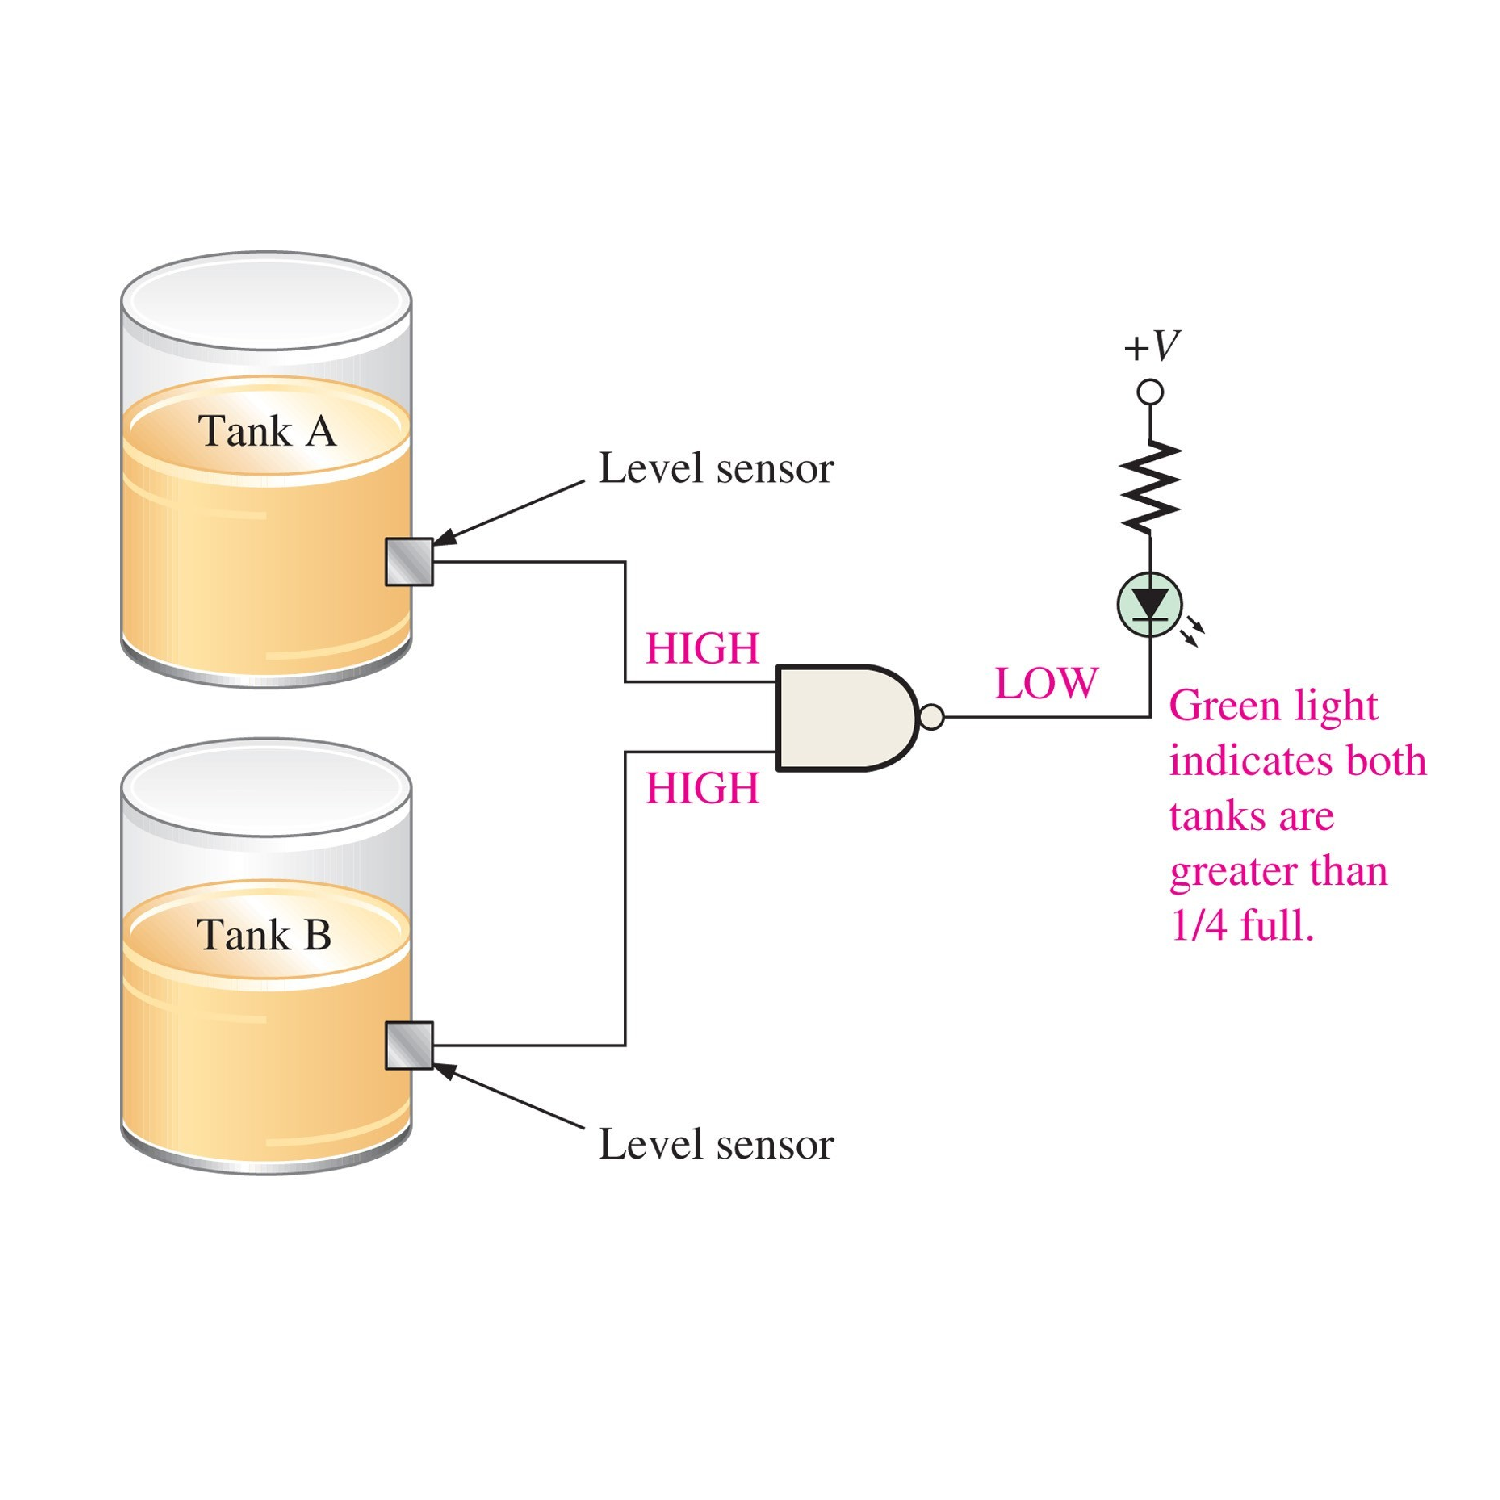
\includegraphics[width=0.25\textwidth]{gateExample6.pdf}
\caption{\label{fig:gates1} (Left) A logic gate combination.  (Right) A liquid tank-level system built from a NAND gate.}
\end{figure}
\begin{enumerate}
\item Generate the simplified logic expression and truth table for Fig. \ref{fig:gates1}, left.  What do you call this type of gate?
\begin{itemize}
\item $out = (\bar{a}+b)(a+\bar{b})$
\item XNOR gate
\end{itemize}
\item Suppose signals $D_{\rm 0}$ and $D_{\rm 1}$ in Fig. \ref{fig:timing7} are connected to $a$ and $b$ in Fig. \ref{fig:gates1}, left.  Generate the timing diagram for $out$. \\ \\ 
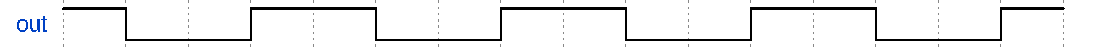
\includegraphics[width=0.9\textwidth]{timingExample8.pdf}
\item \textbf{Creative design}: A liquid tank system is depicted in Fig. \ref{fig:gates1}.  The sensors are HIGH when the liquid is above the level (green ON).  (a) Create a red LED system that activates when both tanks are \textit{below} the level, and draw it below.  (b) Create a yellow LED system that activates when one tank is below and one tank is above the level.  (c) Add a third tank with more liquid, and two pipes guiding liquid to tank A and B.  Each pipe should have a valve.  Add logic that opens the correct valve so as to fill only the low tank until it is no longer below the level.  \\ \\
\begin{itemize}
\item An OR gate with a pull-up resistor connected in series with a red LED.  If S1 and S2 are LOW, then the red LED will light.
\item S1 and S2 input to a XOR gate.  Output connected to a resistor and yellow LED in series to GND.
\item Sensors open valve when they receive a HIGH, and there is an inverter between S1 and its value, and an inverter between S2 and its valve.
\end{itemize}
\end{enumerate}

\clearpage

\section{Chapter 4 - Boolean Algebra and Logic Simplification}
\begin{enumerate}
\item Suppose an investment firm holds stock shares in four different stocks within a portfolio, labled A through D.  The companies corresponding to stocks A through D are labeled \textit{inactive} or \textit{active} by the firm, based on information about their productivity.  The firm notices that the portfolio output is \textit{on} (rising) under the following conditions:
\begin{itemize}
\item All four companies are inactive, or ...
\item Companies A through C are inactive, while company D is active, or ...
\item All companies are active, or ...
\item Companies A through C are active, while company D is inactive.
\end{itemize}
(a) Develop a S-SOP expression for $X$, the portfolio's state (on or off) based on the data above. (b) Use a domain-4 Karnaugh map to simplify the S-SOP expression. (c) Which stock appears to be irrelevant to the state of the portfolio?
\begin{itemize}
\item $X = \bar{A}\bar{B}\bar{C}\bar{D} + \bar{A}\bar{B}\bar{C}D + ABCD + ABC\bar{D}$
\item $X = \bar{A}\bar{B}\bar{C}+ABC$.  The Karnaugh map has two 1's in the upper left, and two 1's in the lower right, forming two S-SOP terms.
\item The D stock is irrelevant to the state of $X$.
\end{itemize}
\item A circuit contains three main branches leading to one output.  The output is observed to fail under the following conditions below.  (a) Use the domain-3 Karnaugh map to determine the conditions under which it does succeed, and write an S-SOP expression for the circuit. (b) Draw the circuit using gates.
\begin{itemize}
\item A: false, B: false, C: false
\item A: false, B: true, C: false
\item A: true, B: true, C: false
\item A: true, B: false, C: false
\item A: false, B: true, C: true
\item A: true, B: true, C: true
\end{itemize}
\begin{itemize}
\item The domain-3 Karnaugh map has two true states: upper right corner and lower-right corner.  $X=\bar{B}C$.
\item B goes into an inverter, then an AND, along with C.
\end{itemize}
\end{enumerate}

\section{Chapter 5 - Combinatorial Logic Analysis}
\label{sec:comb}
\begin{figure}[ht]
\centering
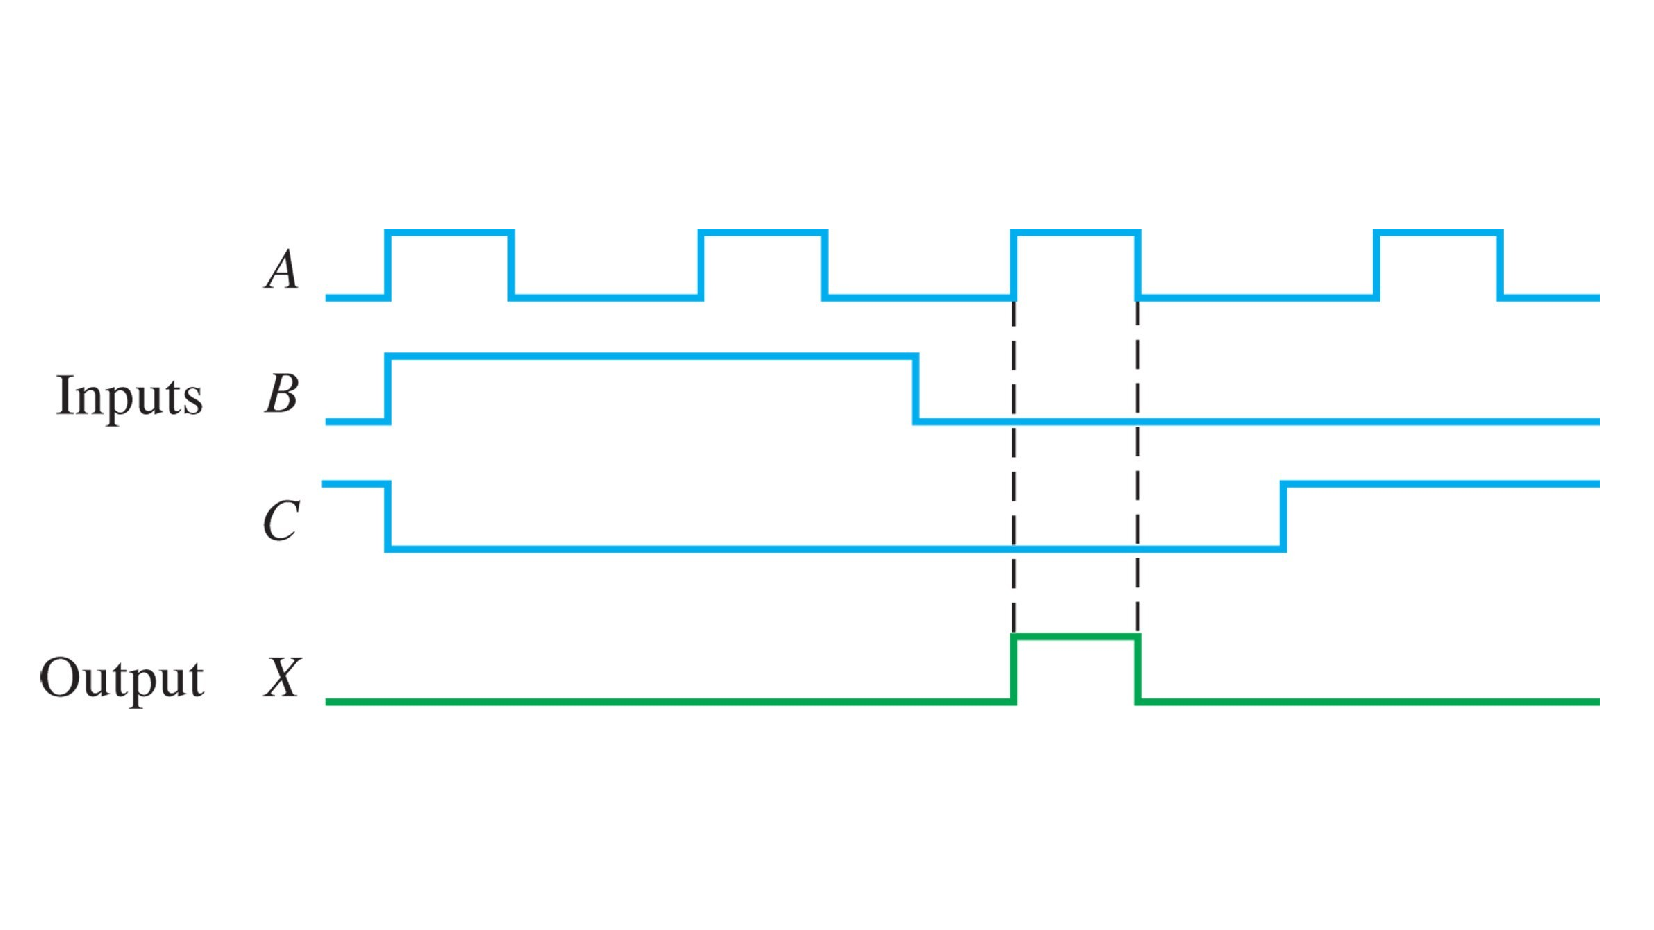
\includegraphics[width=0.4\textwidth,trim=0cm 3cm 0cm 2cm,clip=true]{timingExample7.pdf}
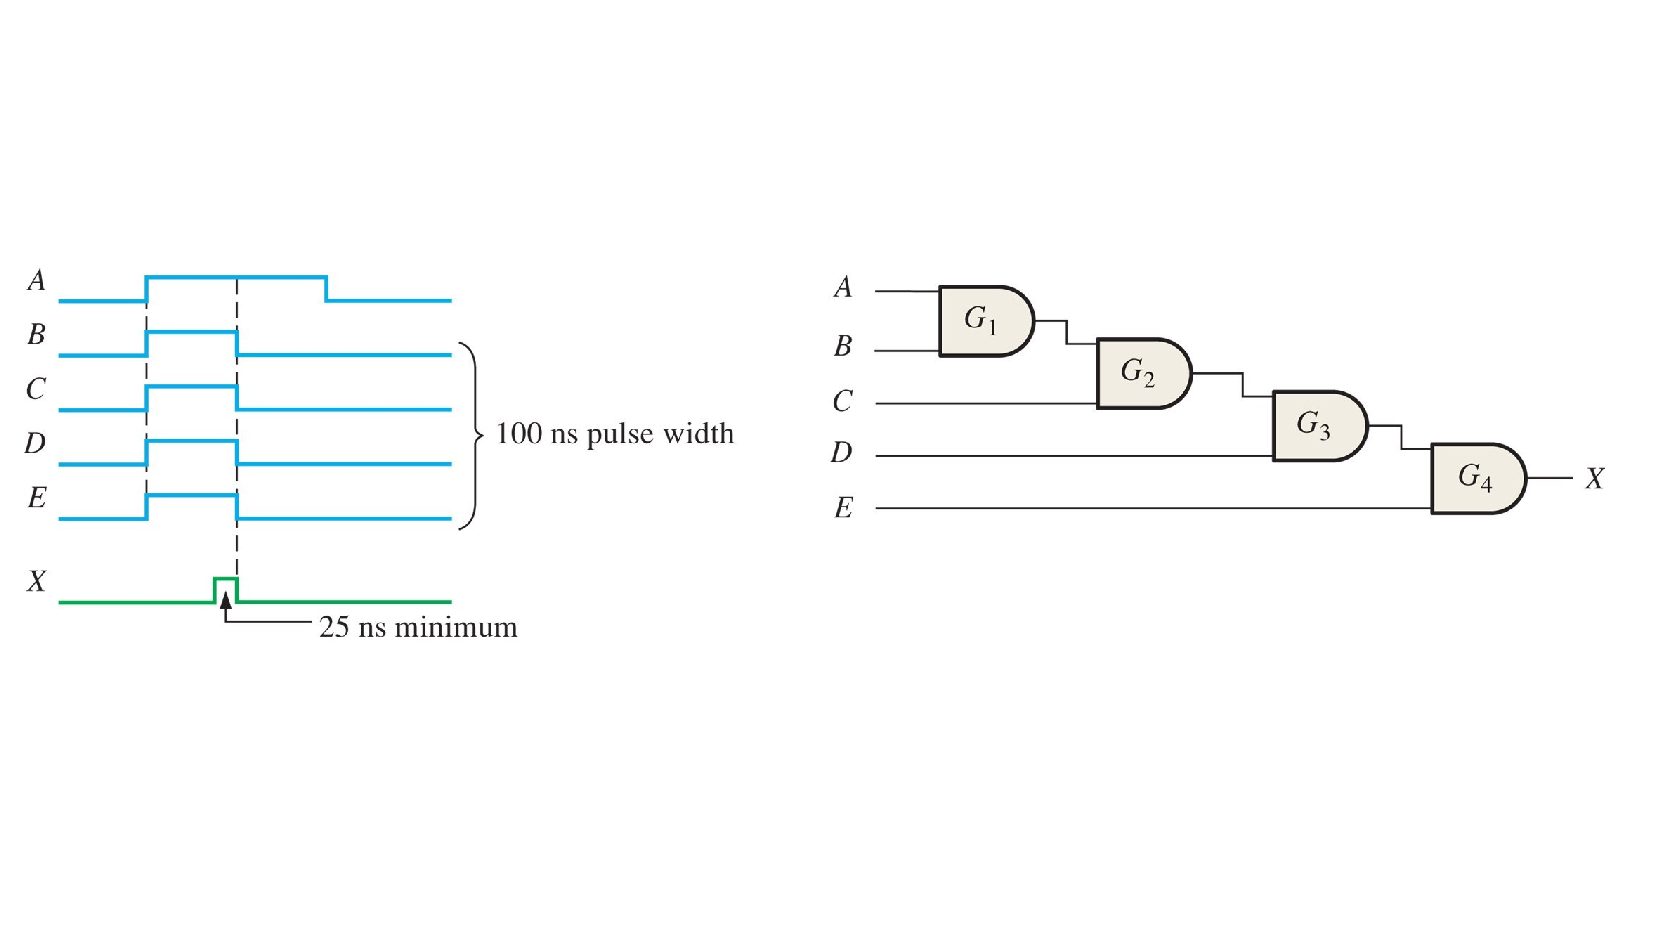
\includegraphics[width=0.5\textwidth,trim=0cm 4cm 0cm 2cm,clip=true]{bonus.pdf}
\caption{\label{fig:timing3} Diagrams for Sec. \ref{sec:comb}. (Left) Inputs are ABC, and the output is X. (Right) The inputs are ABCDE, and the output is X.}
\end{figure}
\begin{enumerate}
\item For the input waveforms shown in Fig. \ref{fig:timing3} (left), what logic circuit will generate the output waveform? \\ \\
$X = A\bar{B}\bar{C}$ (Two inverters: one for B, one for C.  One 3-inpput AND gate.
\item \textbf{Bonus}: Assumming a propagation delay of 10 ns through each gate in Fig. \ref{fig:timing3}, determine if the \textit{desired} output waveform X will be generated.  The desired output is a pulse with a minimum width of 25 ns. \\ \\
Yes, the waveform will be wide enough given the propagation delays in the gates.
\end{enumerate}

\end{document}